
\begin{figure}[htbp]
    \centering
    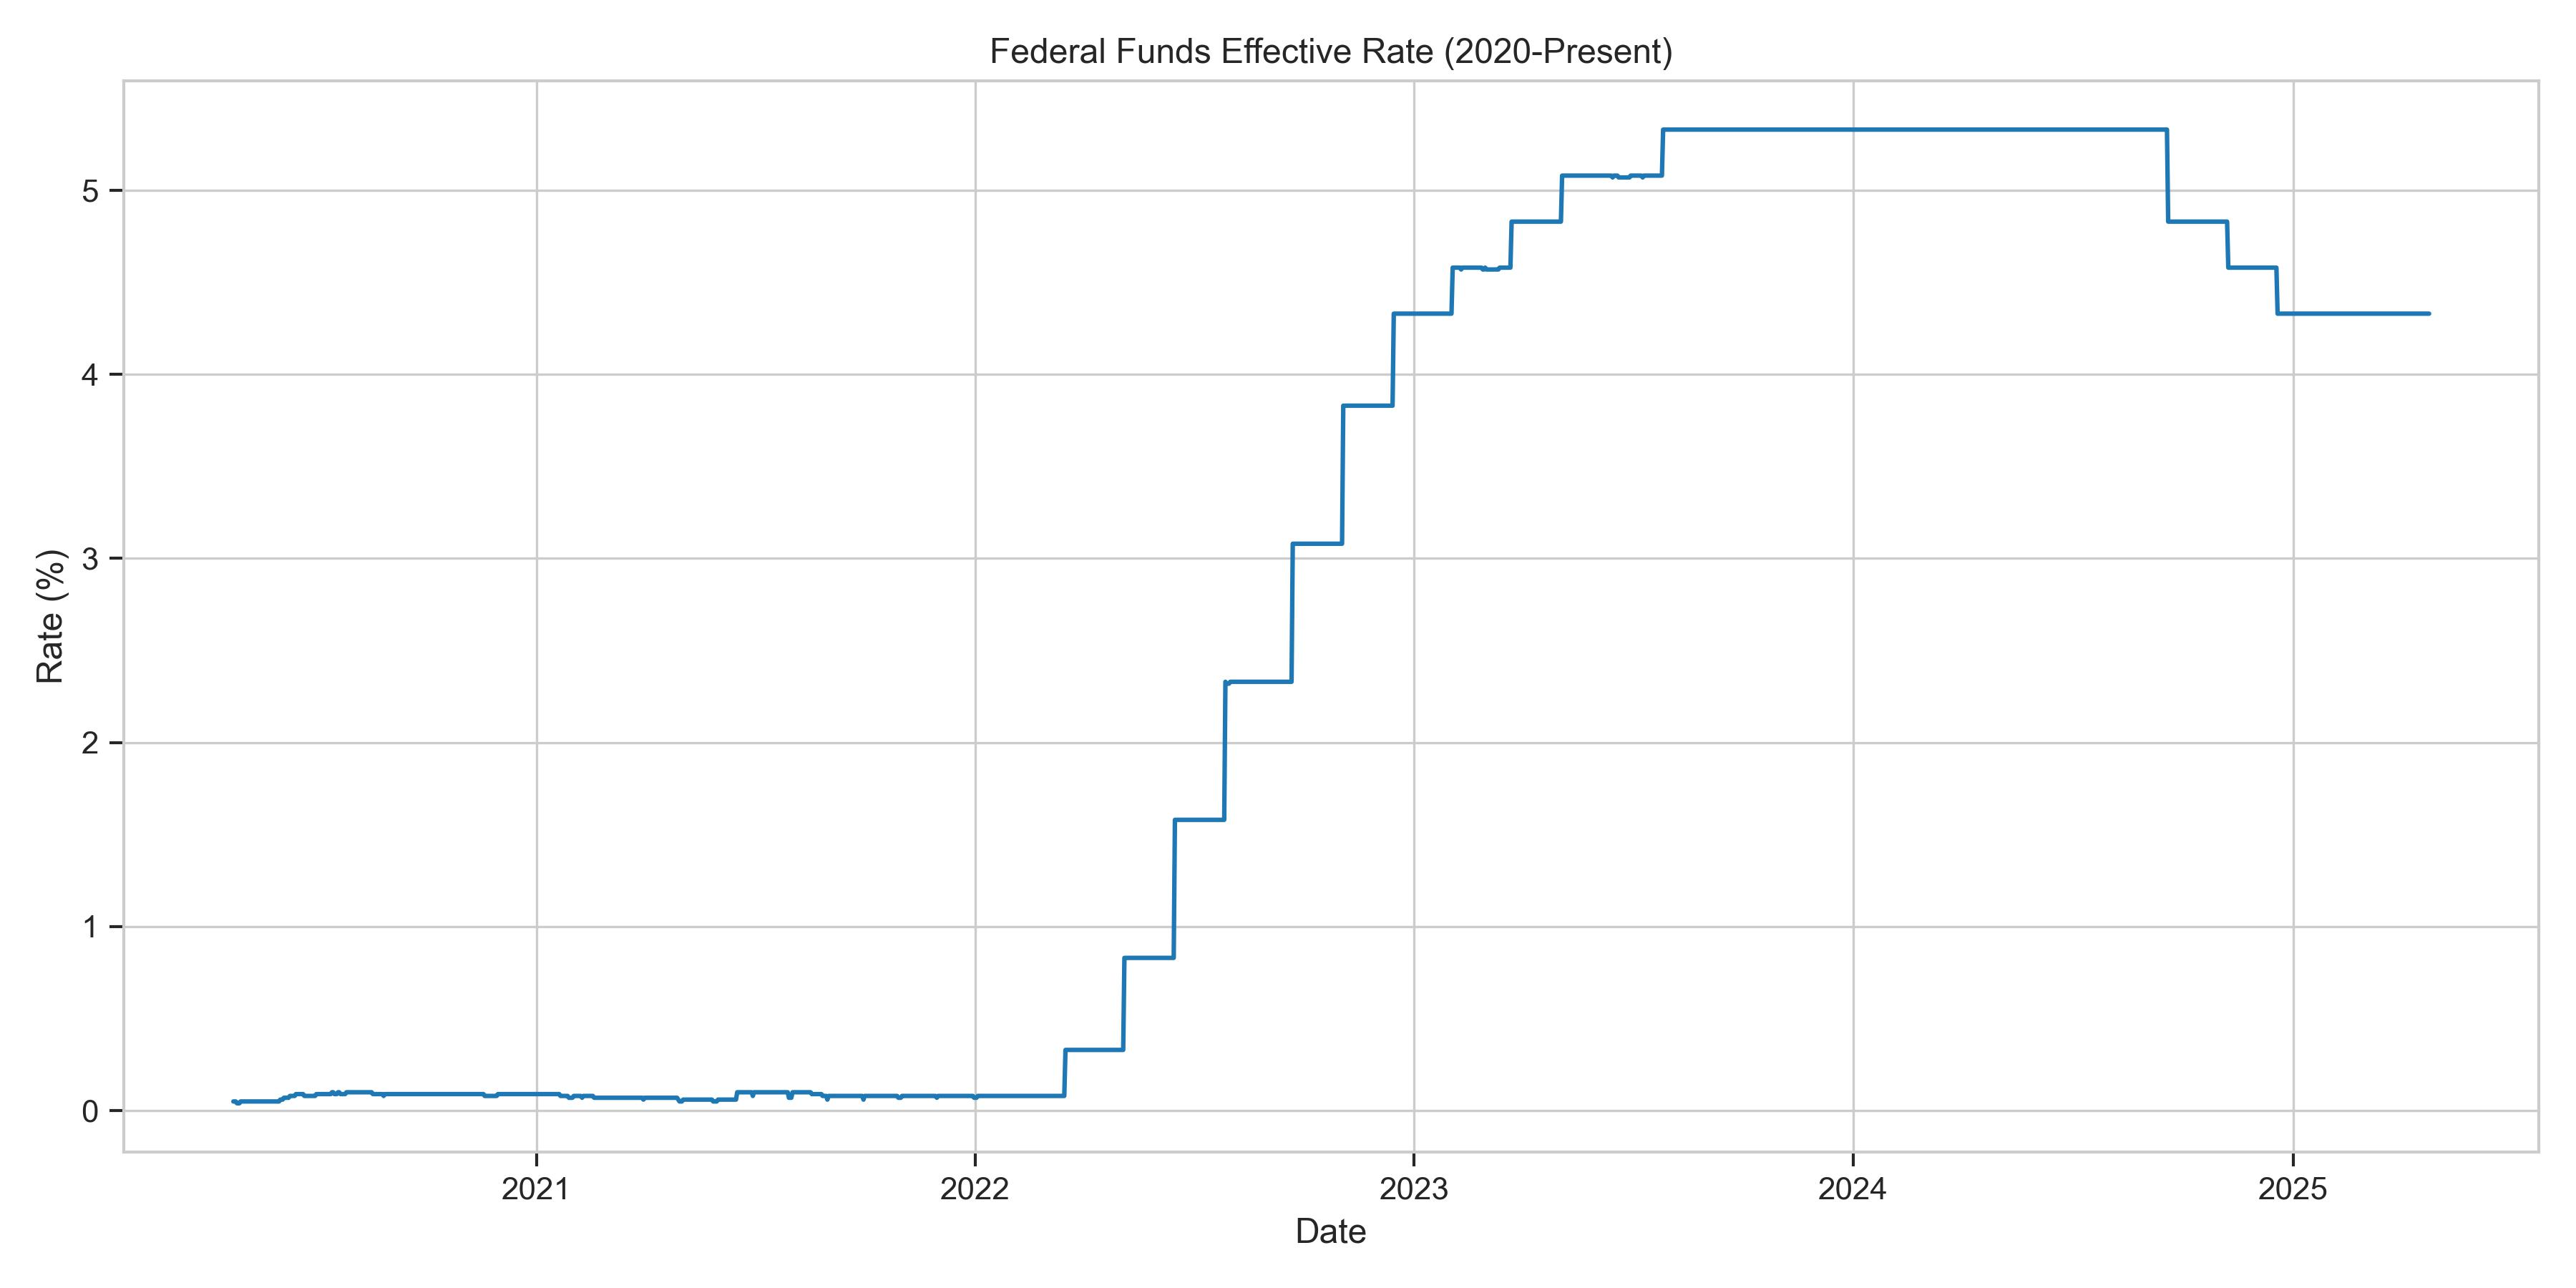
\includegraphics[width=\textwidth]{figure1_ff_rate_timeseries.jpg}
    \caption{Federal Funds Effective Rate time series (2020-Present)}
    \label{fig:ff_rate_timeseries}
\end{figure}

\begin{figure}[htbp]
    \centering
    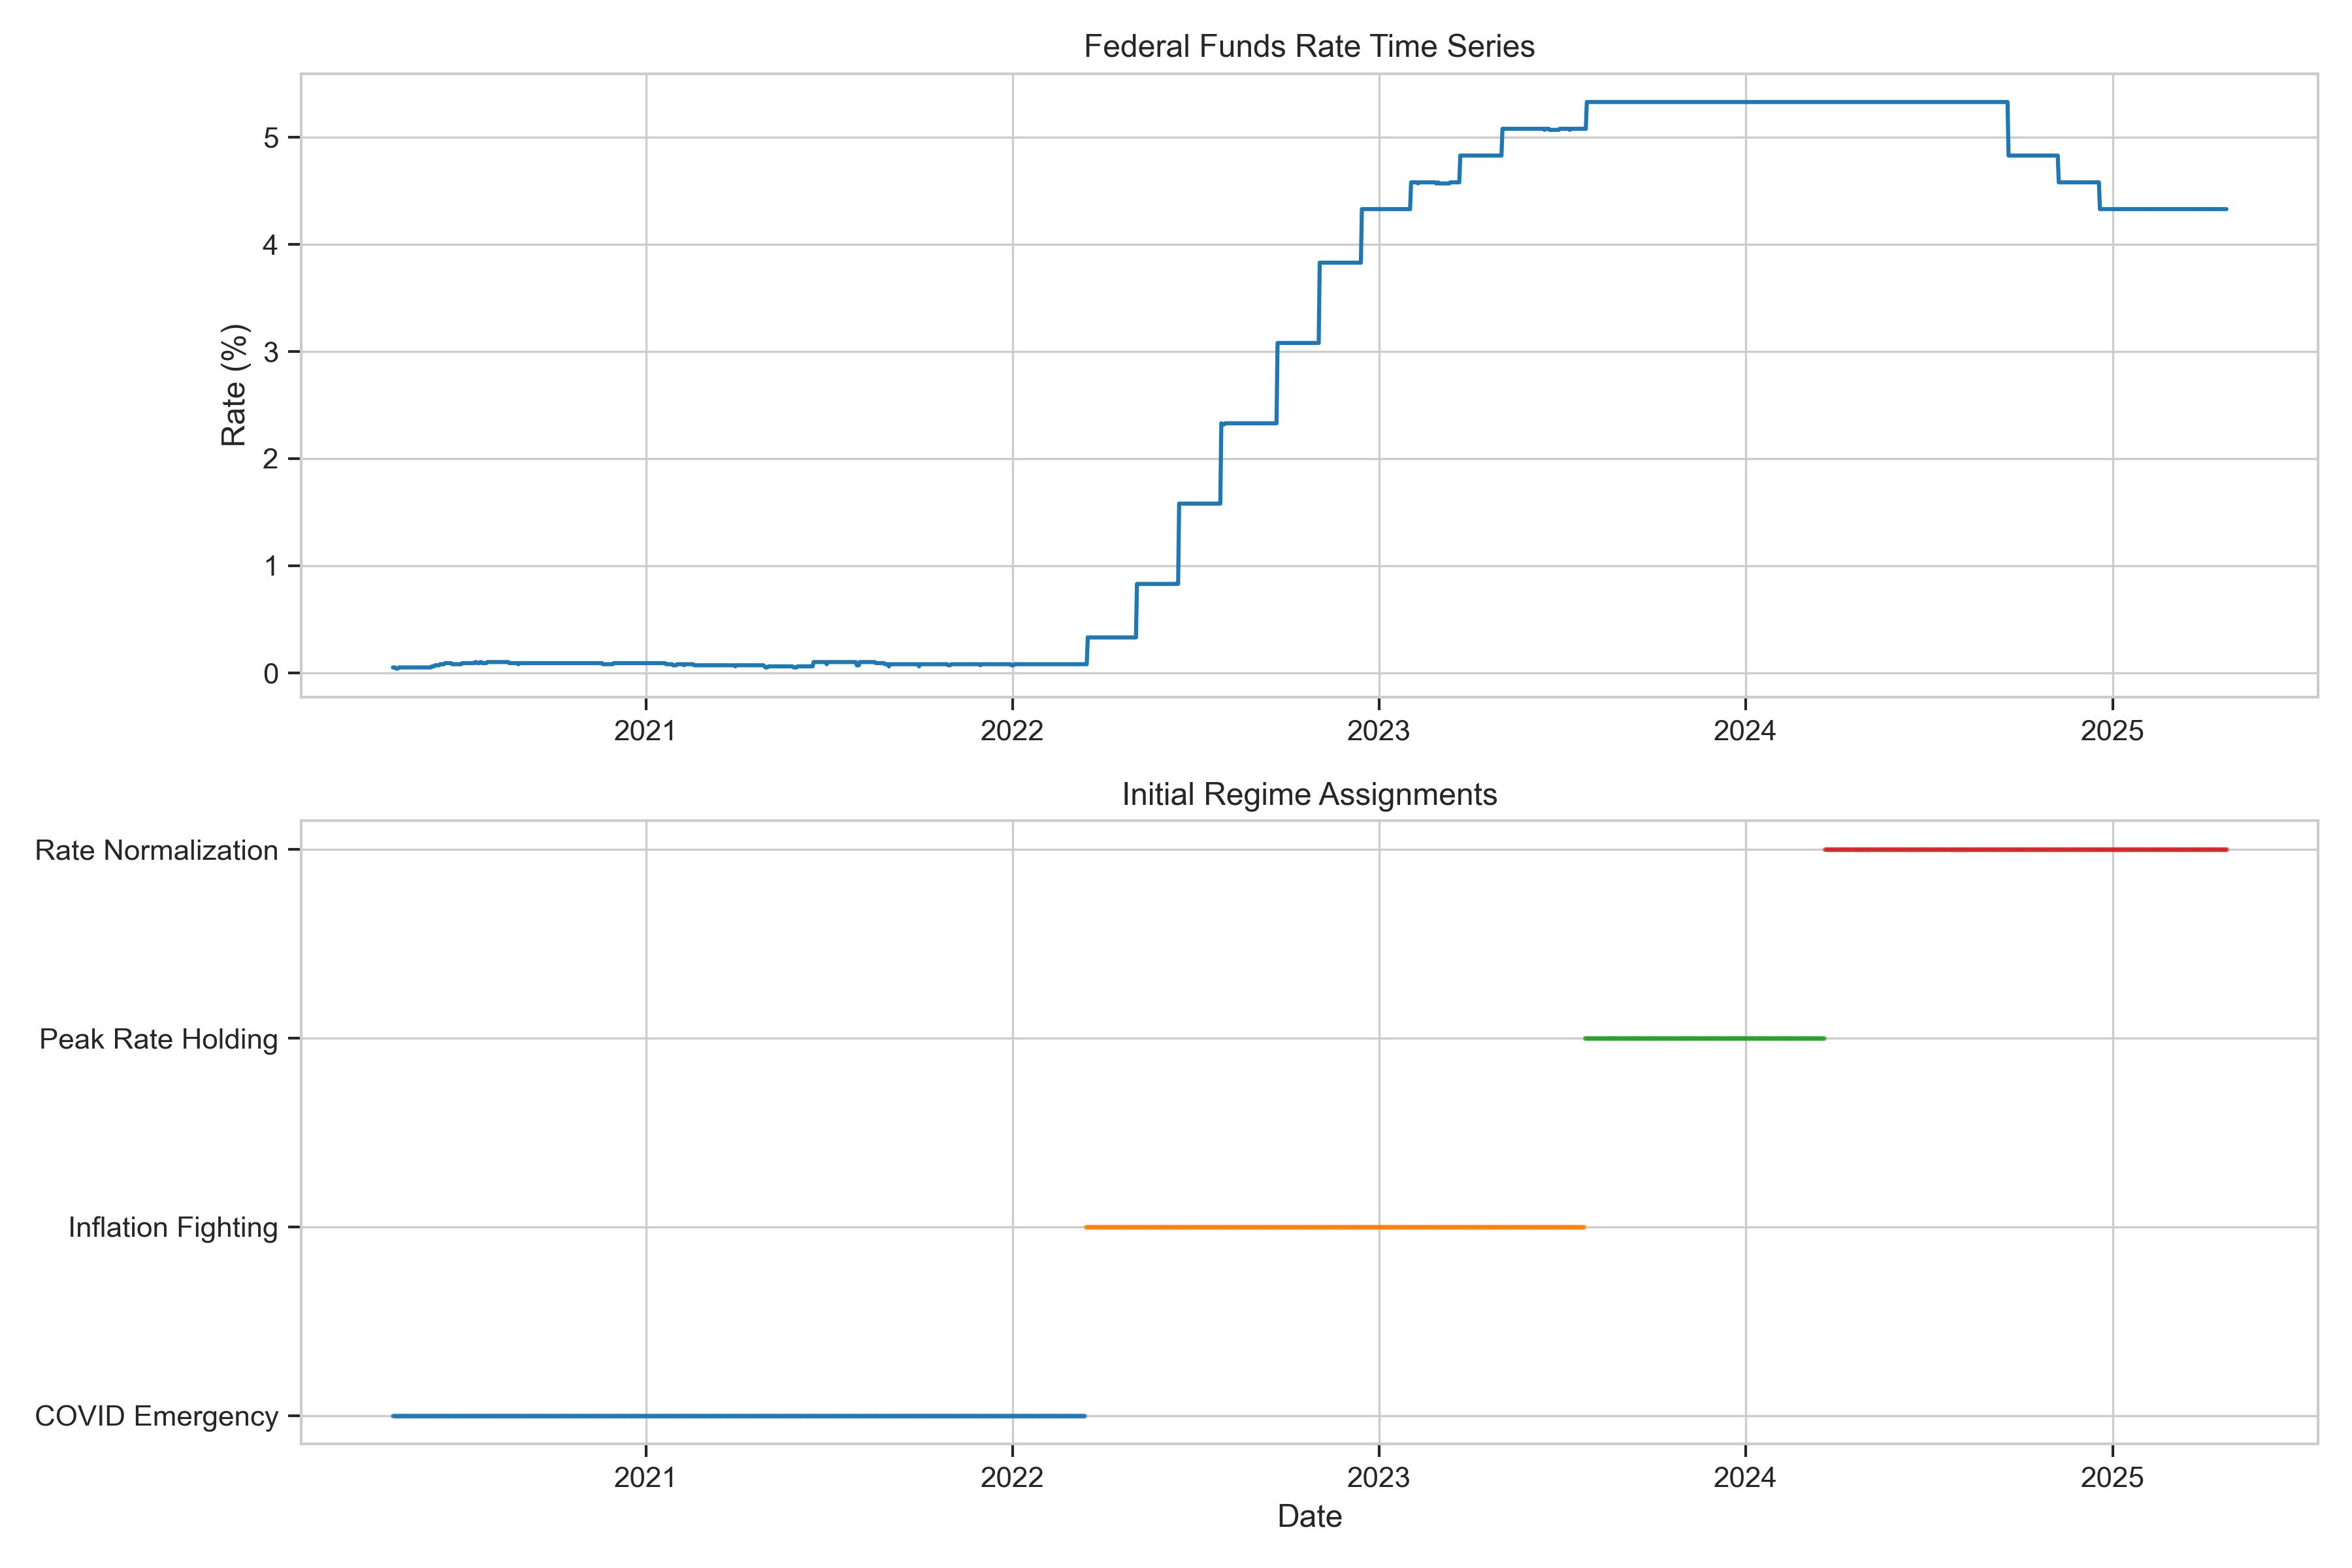
\includegraphics[width=\textwidth]{figure2_initial_regimes.jpg}
    \caption{Initial regime assignments based on simple change point detection}
    \label{fig:initial_regimes}
\end{figure}

\begin{figure}[htbp]
    \centering
    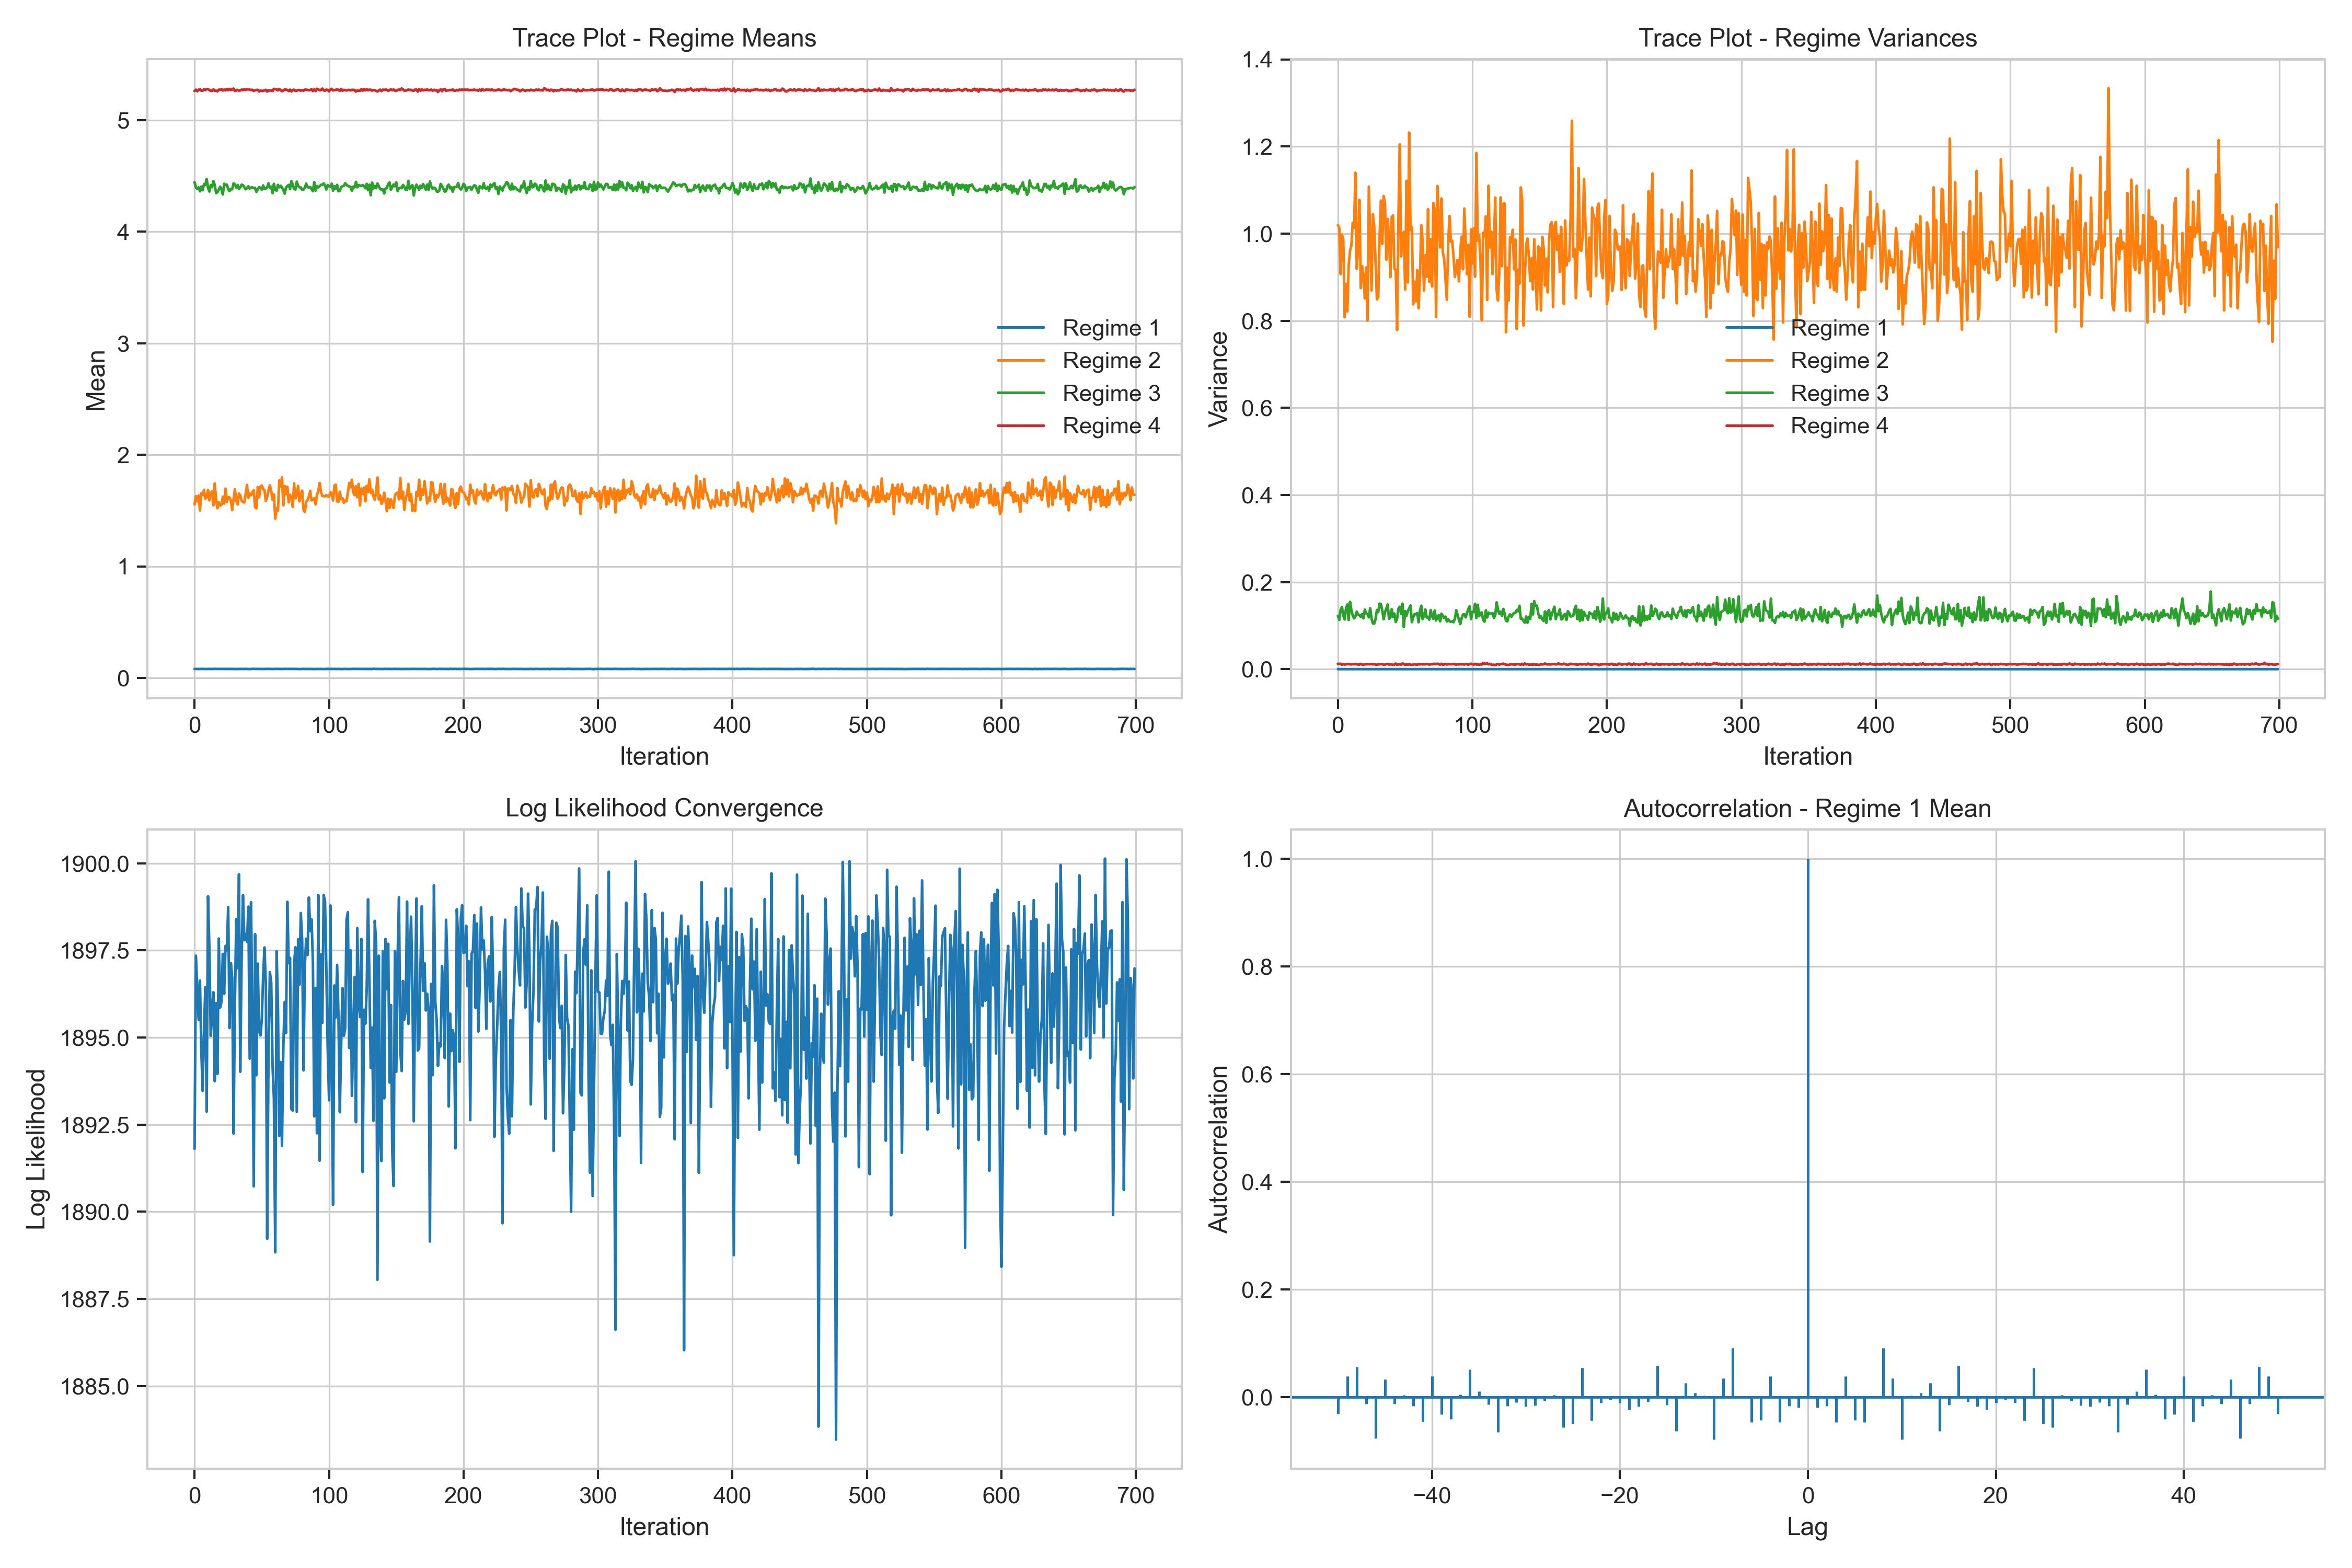
\includegraphics[width=\textwidth]{figure3_informative_priors_convergence.jpg}
    \caption{MCMC Convergence Diagnostics for the Informative Priors model. Top: Trace plots for regime means (left) and variances (right). Bottom: Log likelihood convergence (left) and autocorrelation (right).}
    \label{fig:convergence}
\end{figure}

\begin{figure}[htbp]
    \centering
    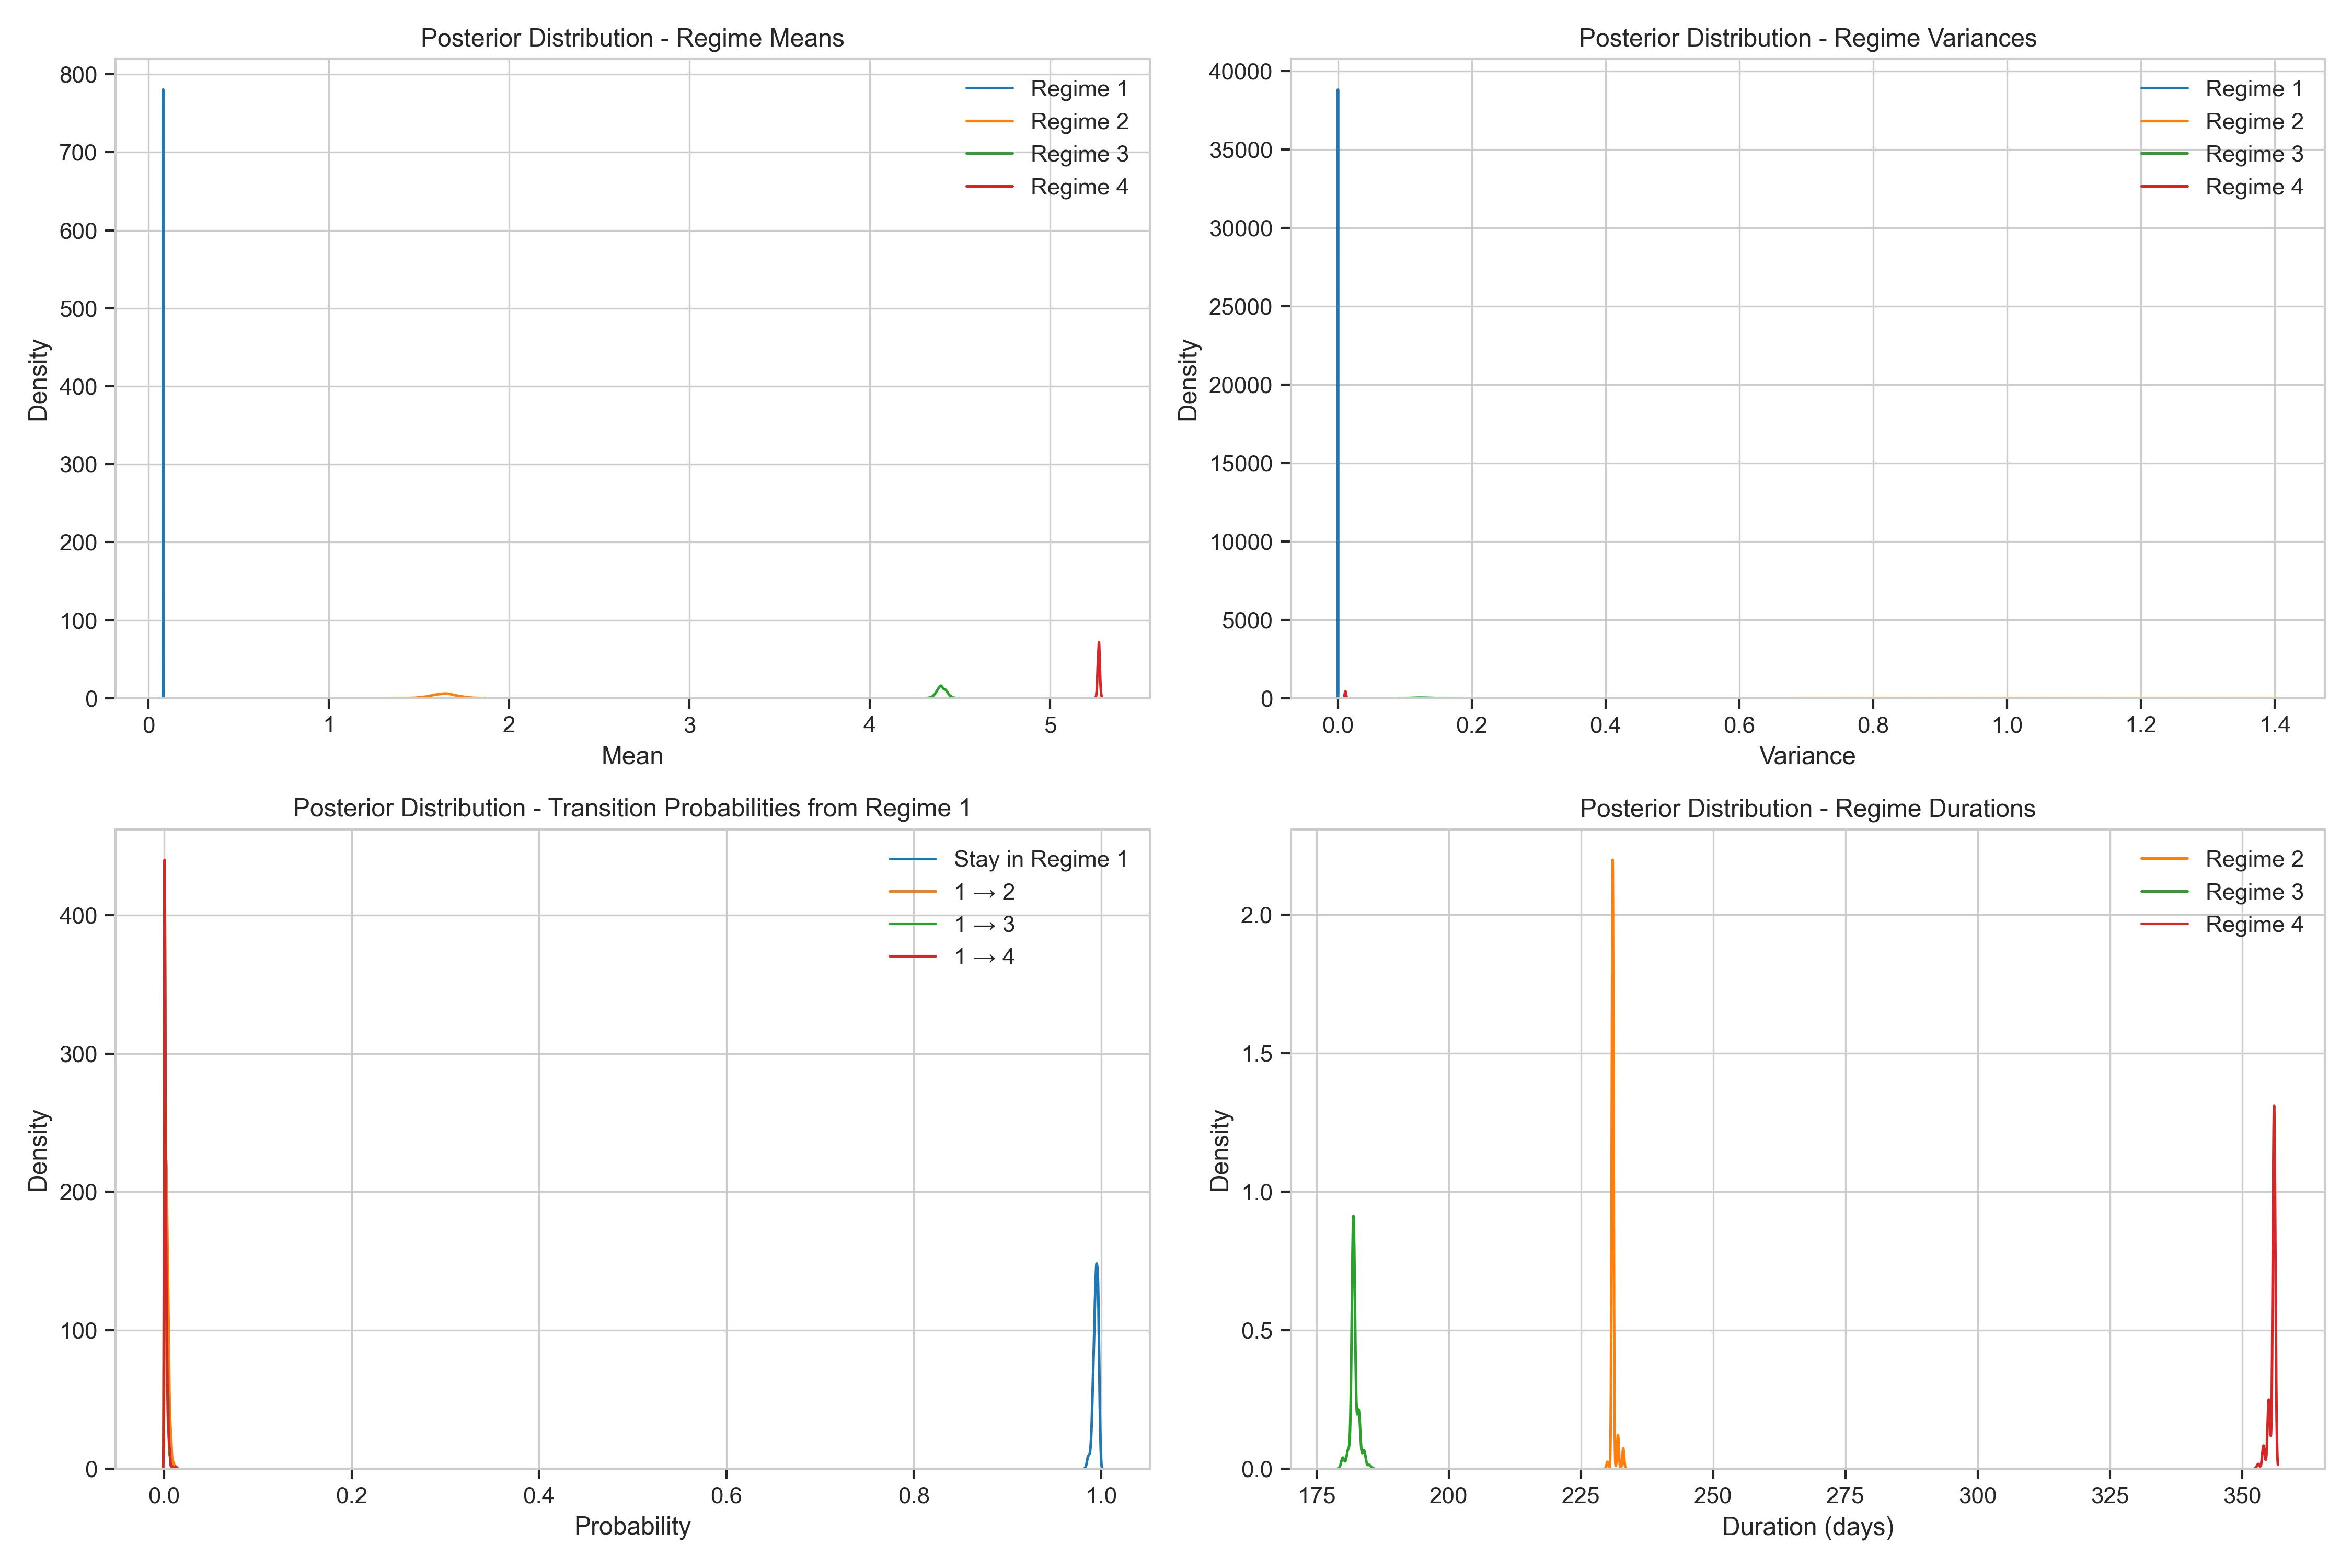
\includegraphics[width=\textwidth]{figure4_informative_priors_posteriors.jpg}
    \caption{Posterior Distributions for the Informative Priors model. Top: Regime means (left) and variances (right). Bottom: Transition probabilities from Regime 1 (left) and regime durations (right).}
    \label{fig:posteriors}
\end{figure}

\begin{figure}[htbp]
    \centering
    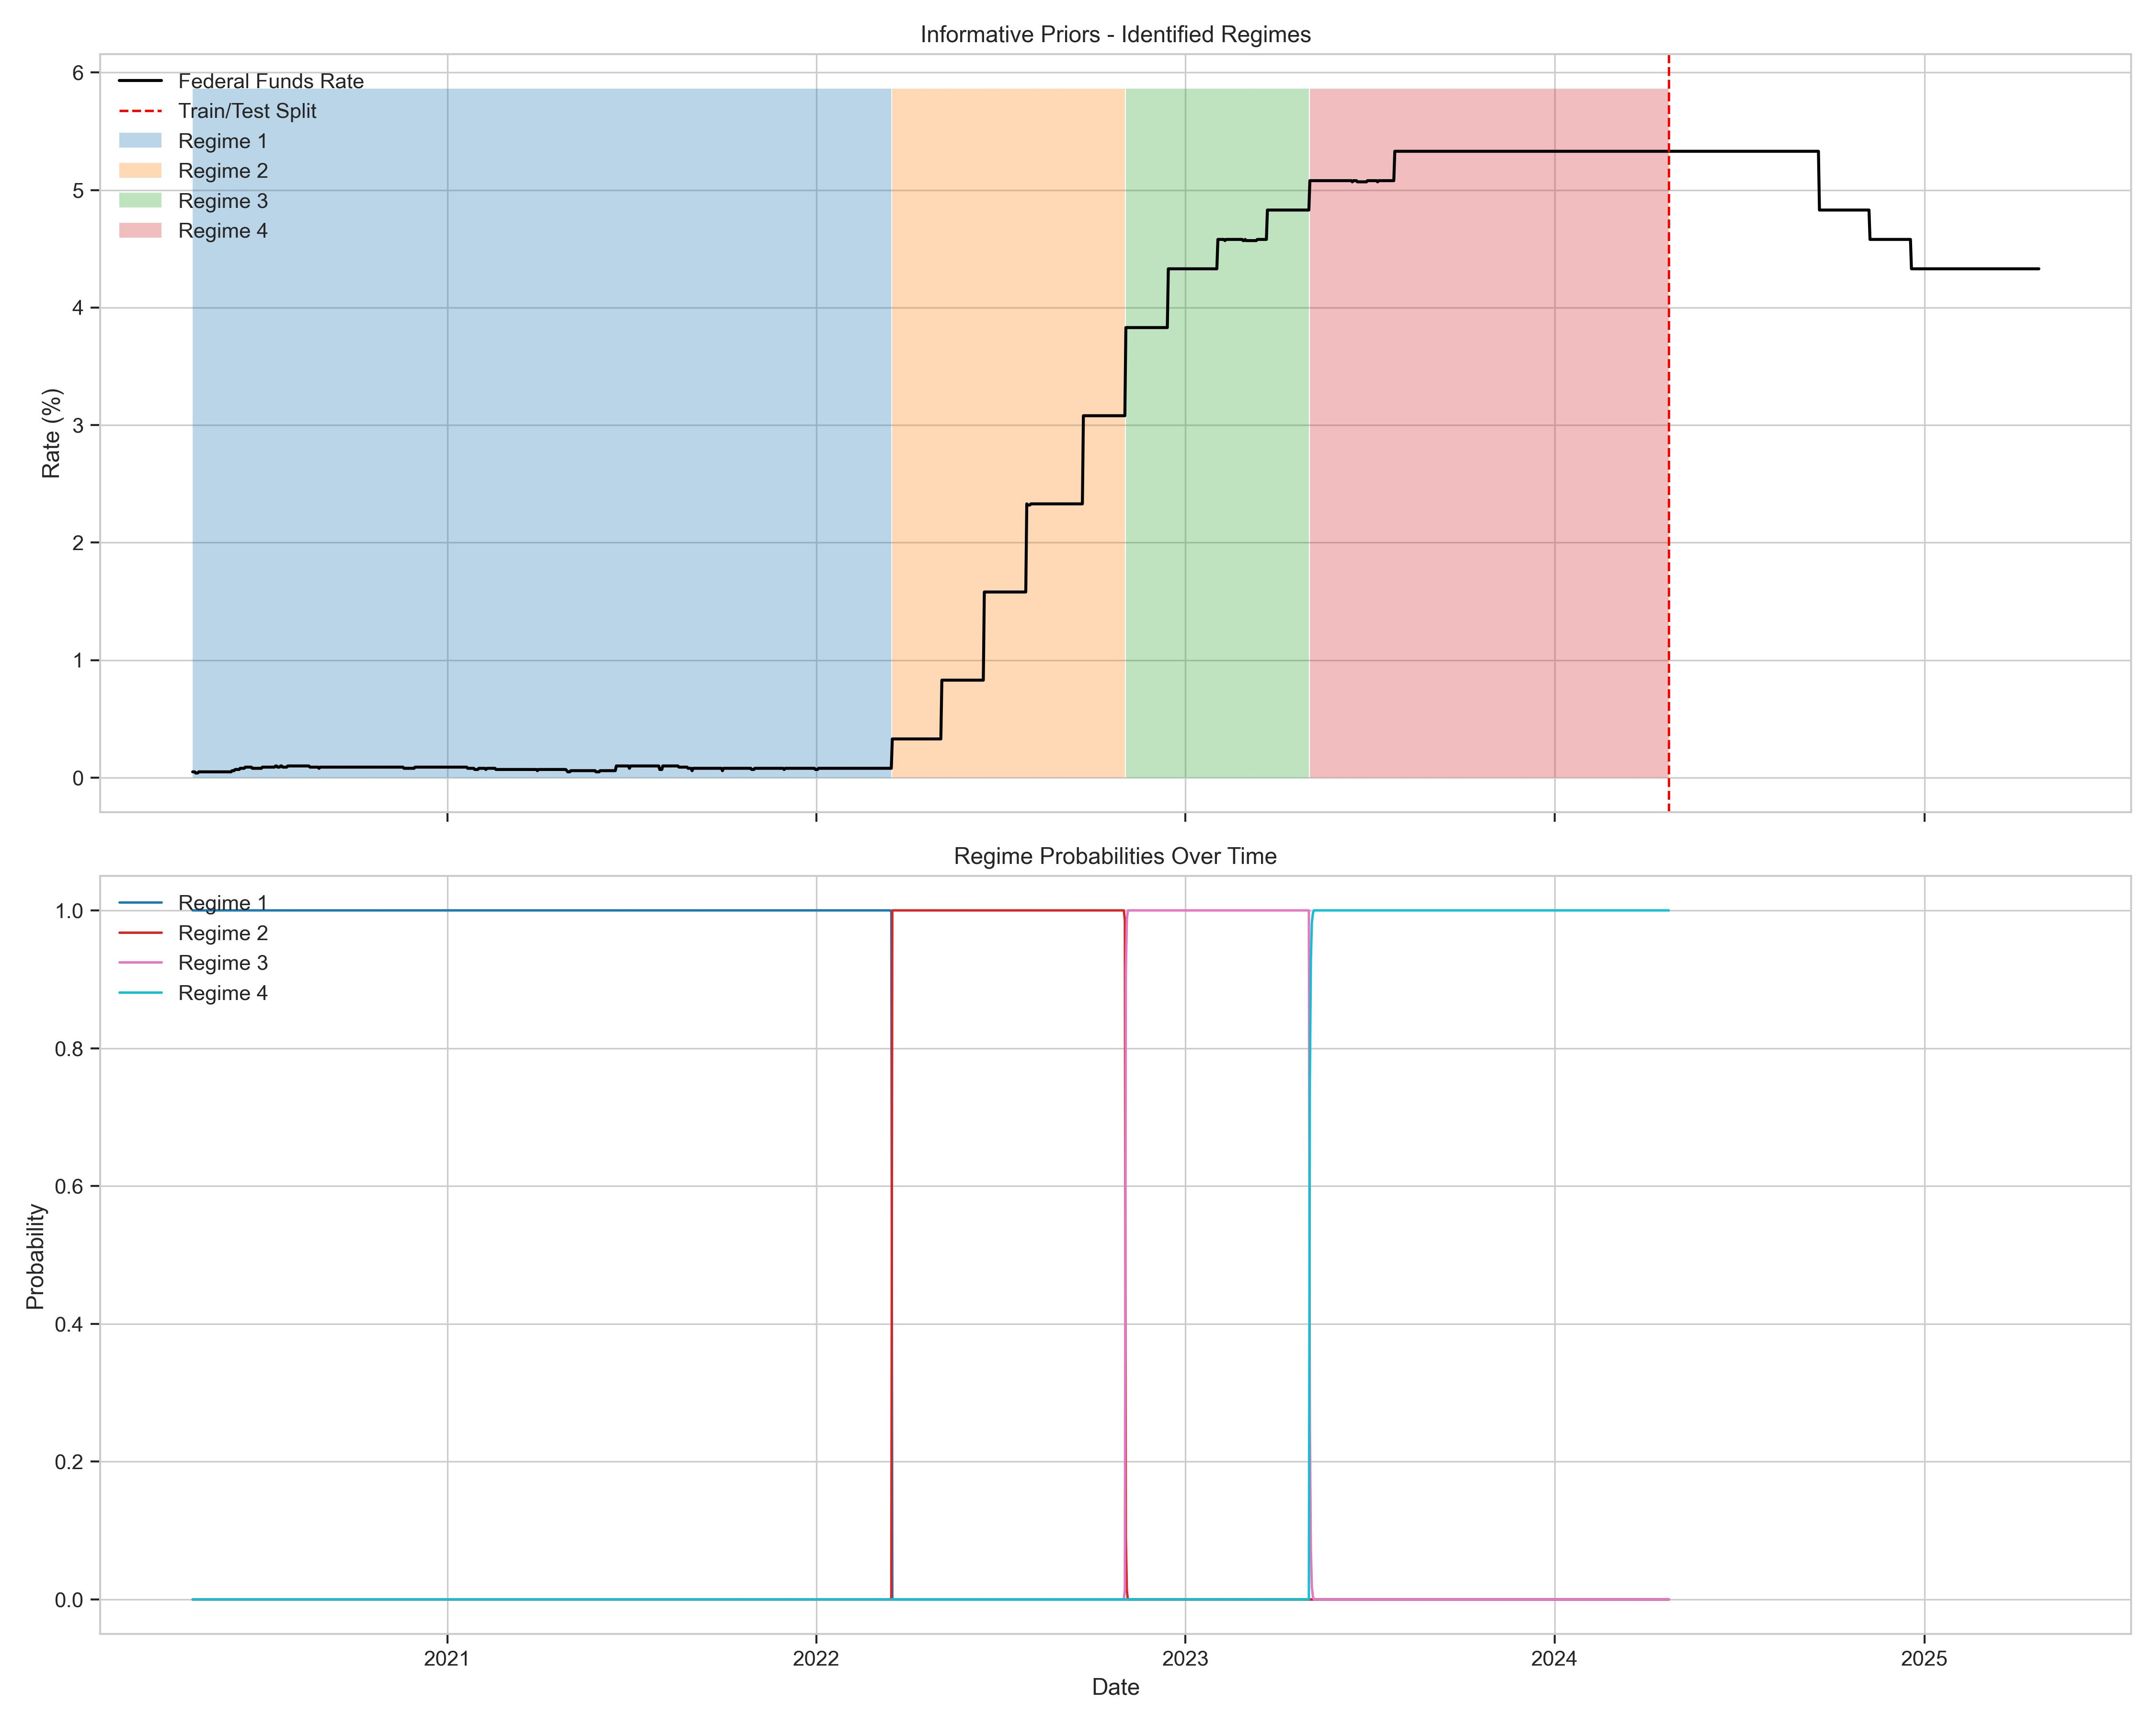
\includegraphics[width=\textwidth]{figure5_informative_priors_regimes.jpg}
    \caption{Identified regimes (top) and regime probabilities over time (bottom) for the Informative Priors model.}
    \label{fig:regimes}
\end{figure}

\begin{figure}[htbp]
    \centering
    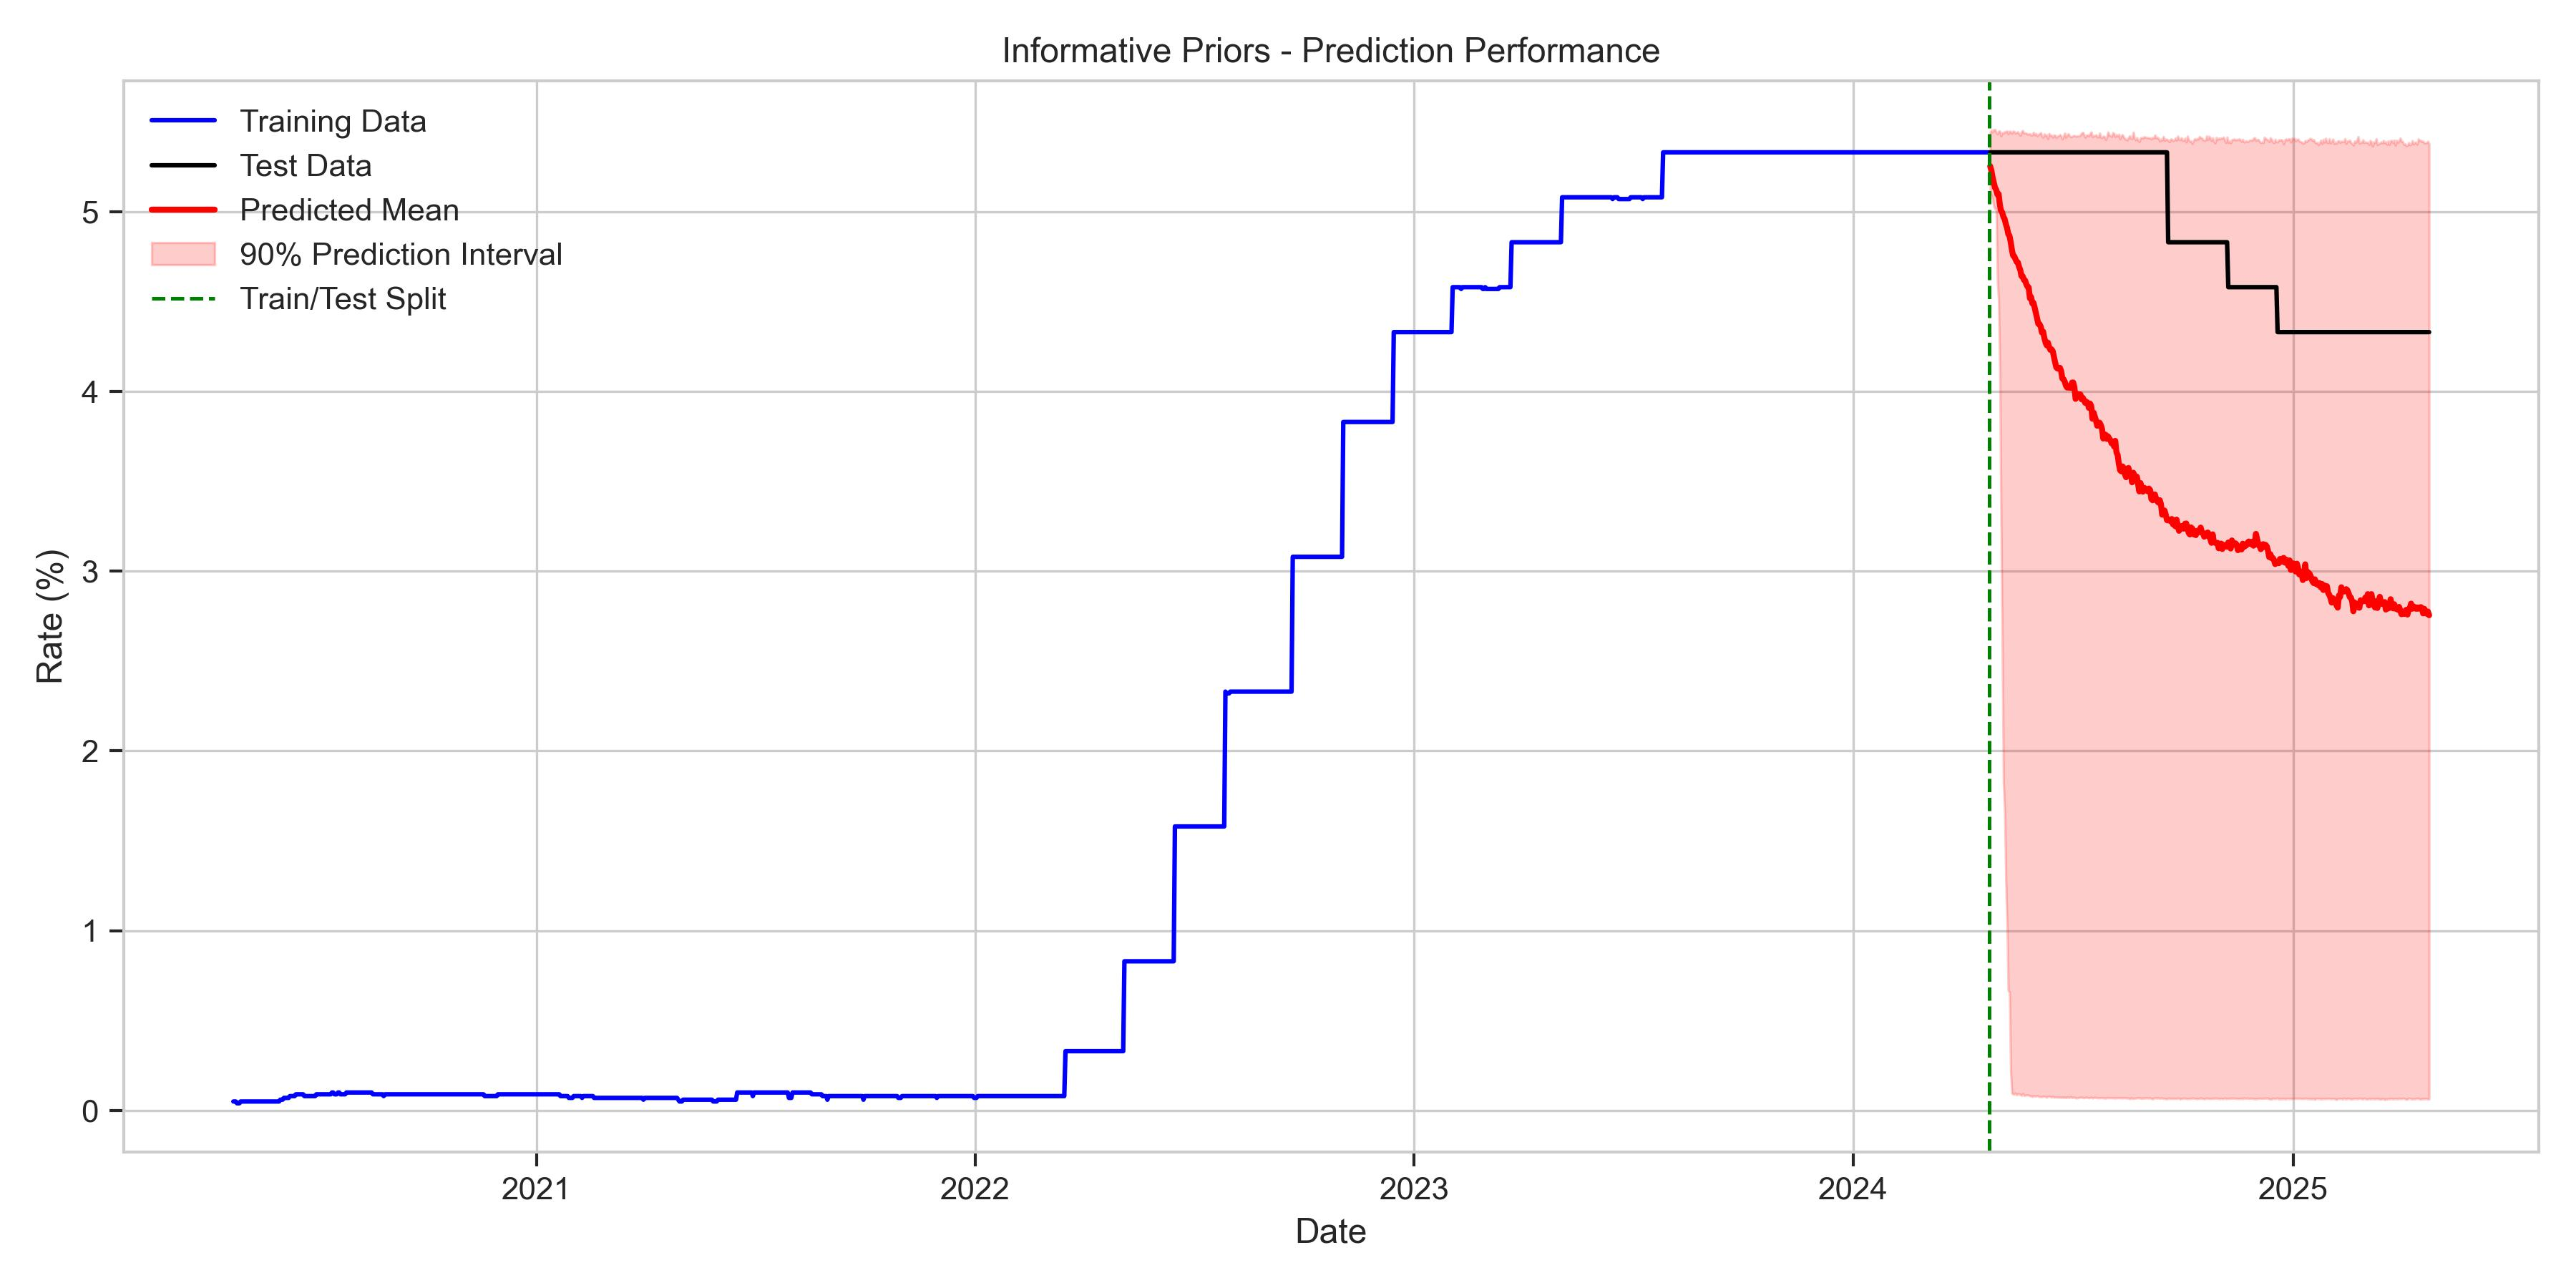
\includegraphics[width=\textwidth]{figure6_informative_priors_prediction.jpg}
    \caption{Prediction performance of the Informative Priors model with 90\% prediction intervals.}
    \label{fig:prediction}
\end{figure}

\begin{figure}[htbp]
    \centering
    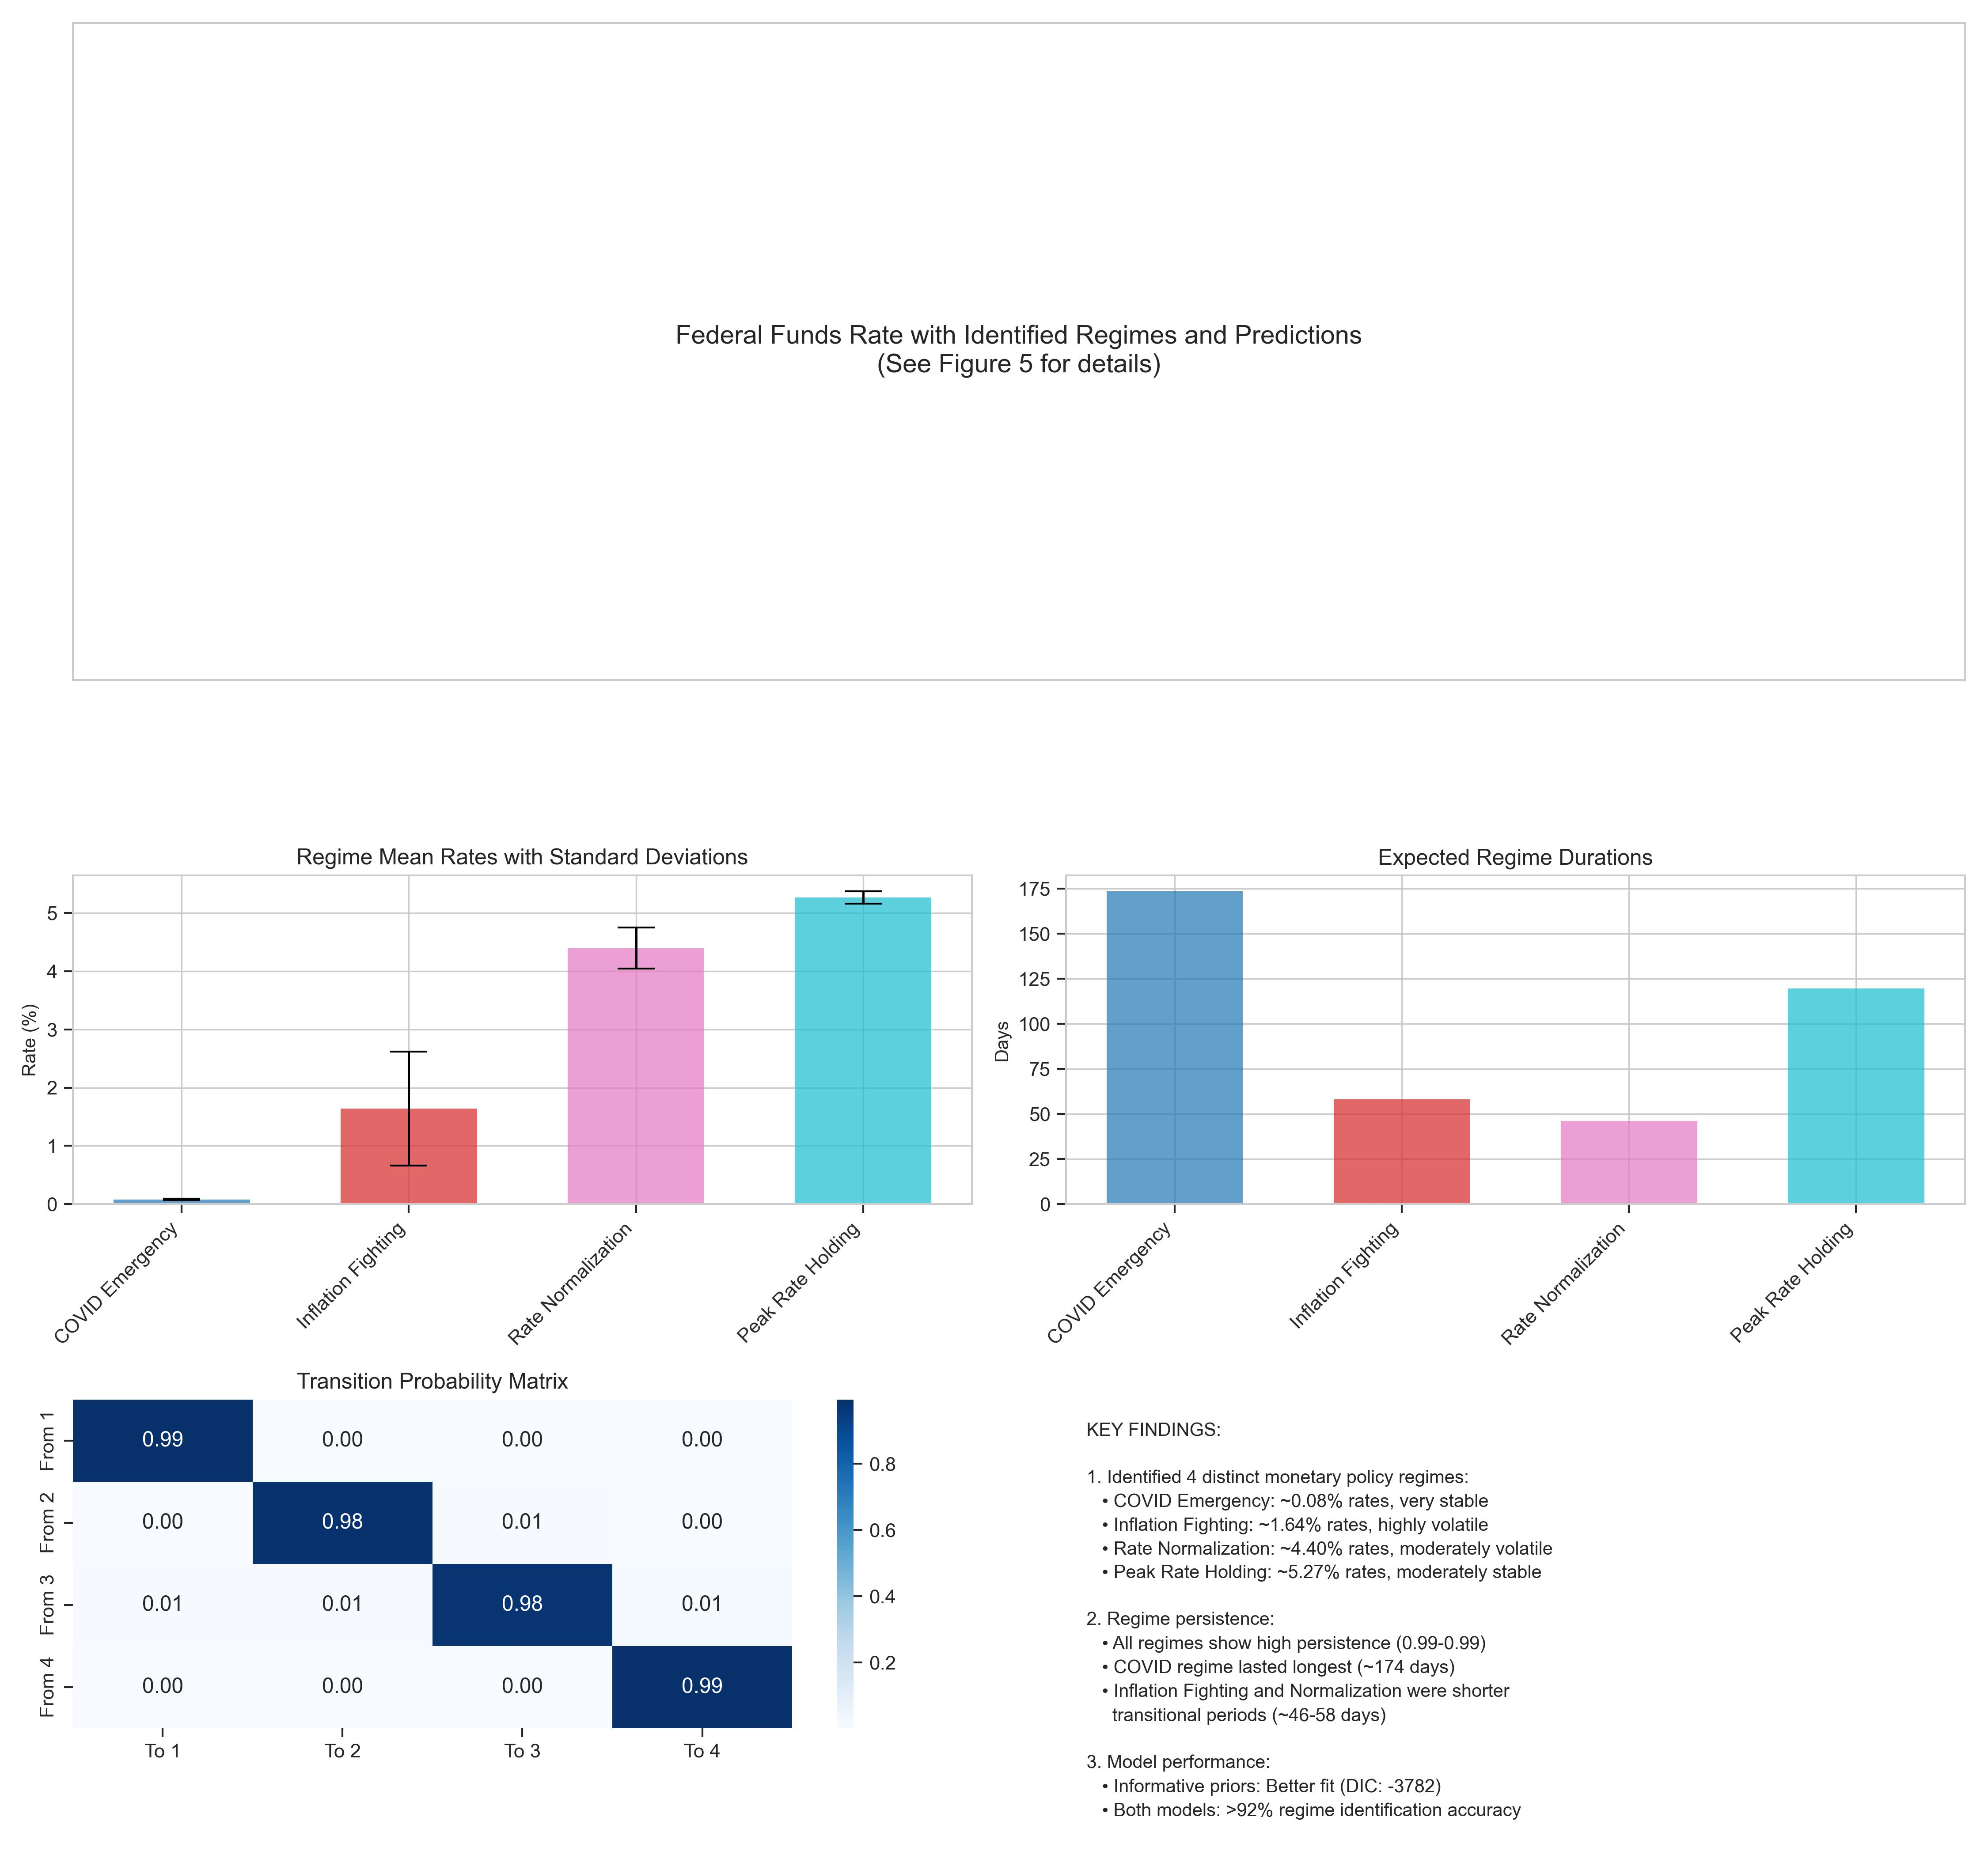
\includegraphics[width=\textwidth]{figure7_final_summary_visualization.jpg}
    \caption{Summary visualization of the Federal Funds Rate regime analysis, showing regime characteristics and key findings.}
    \label{fig:summary}
\end{figure}

\begin{figure}[htbp]
    \centering
    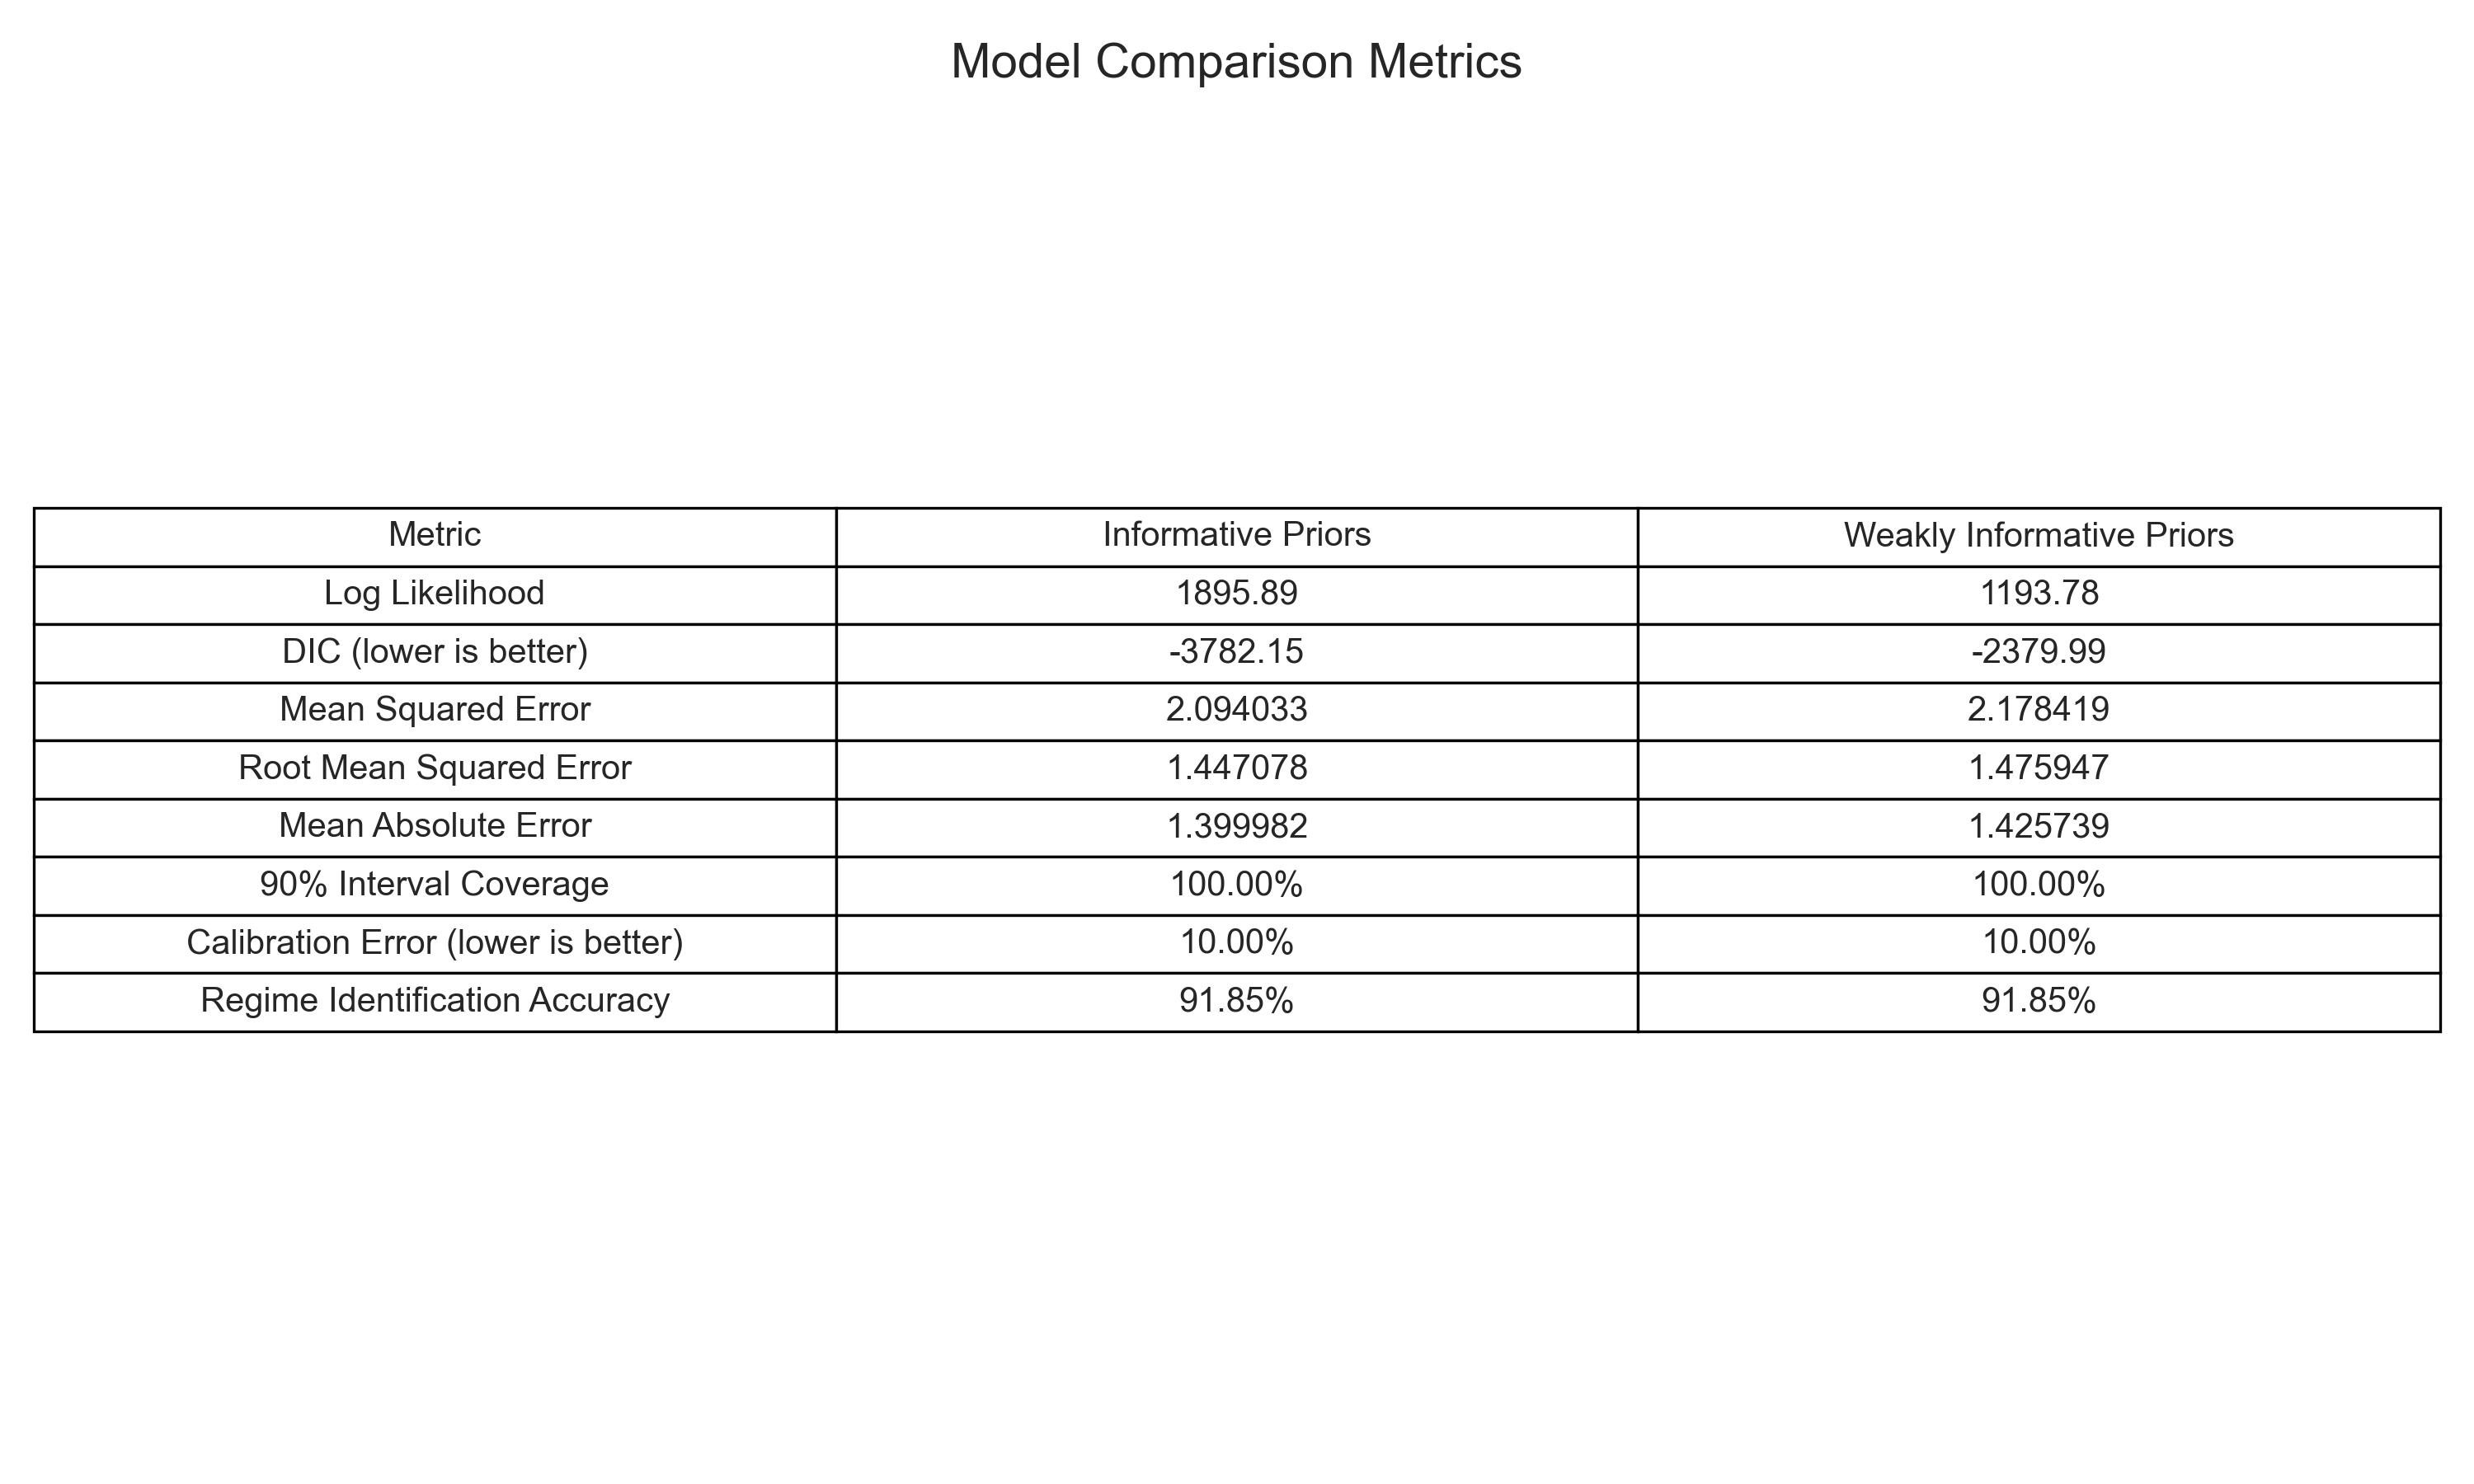
\includegraphics[width=\textwidth]{figure8_model_comparison_table.jpg}
    \caption{Comparison of model performance metrics between Informative and Weakly Informative priors.}
    \label{fig:comparison_table}
\end{figure}

\begin{figure}[htbp]
    \centering
    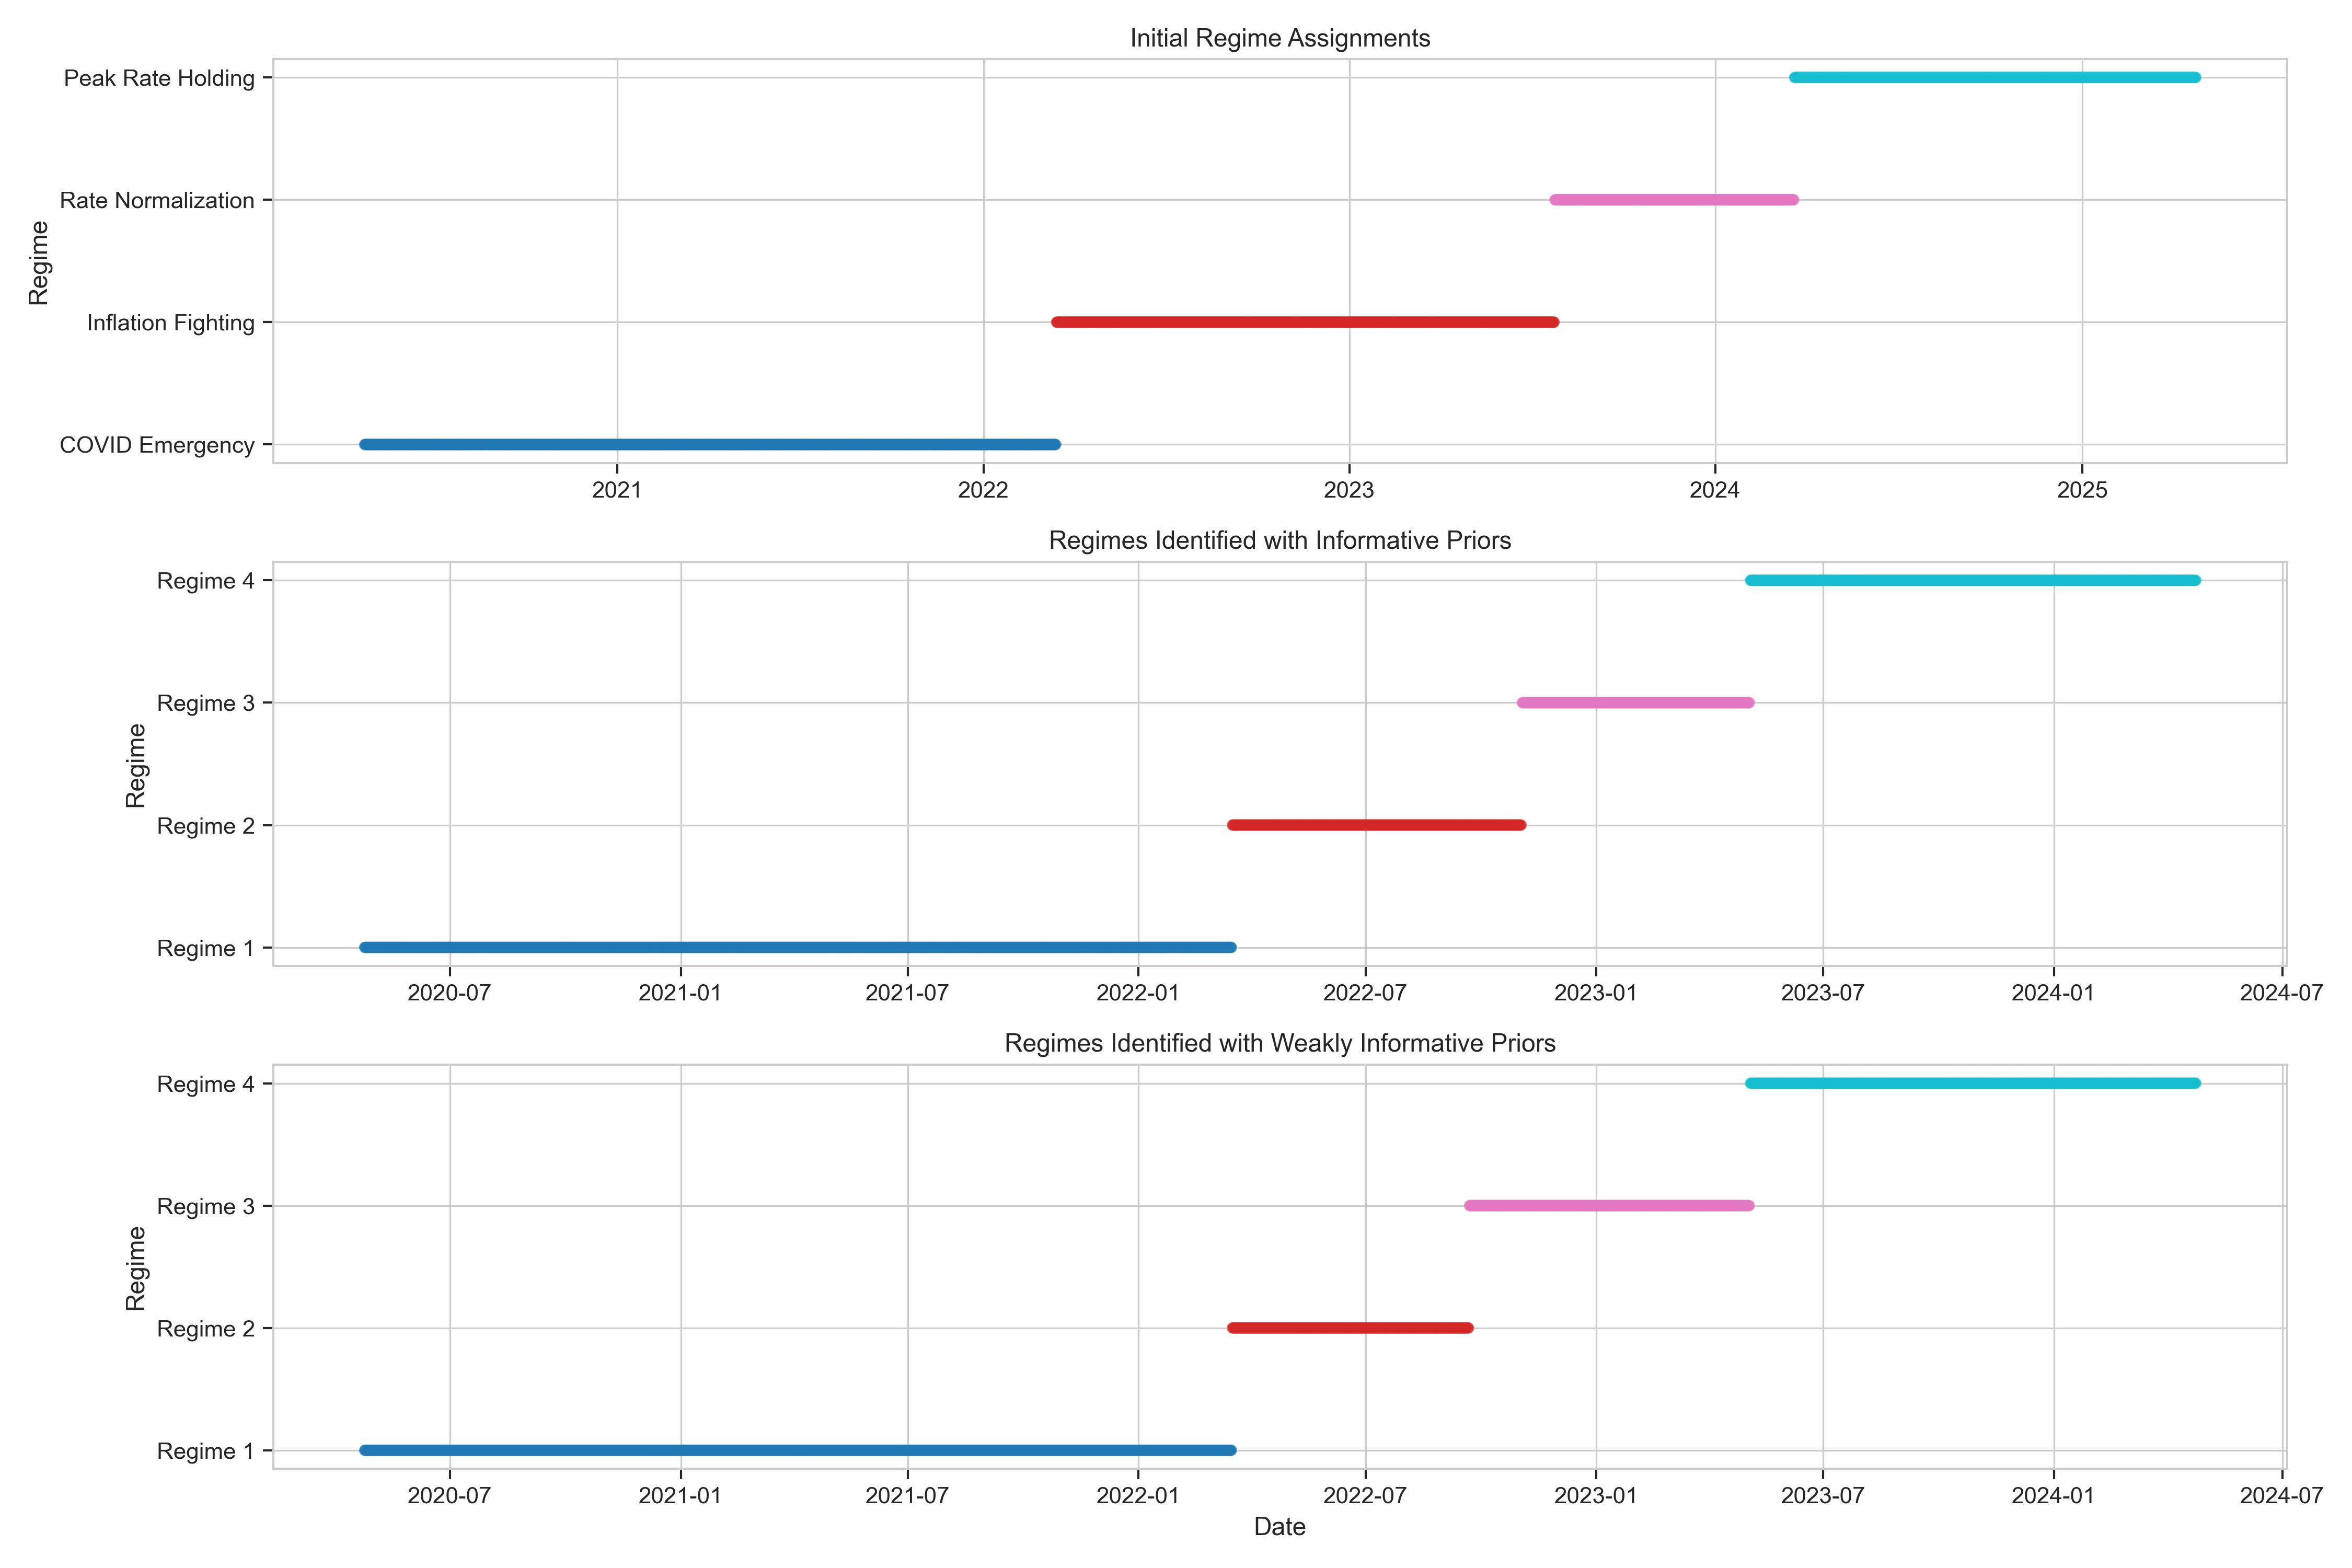
\includegraphics[width=\textwidth]{figure9_model_comparison_regimes.jpg}
    \caption{Comparison of regime assignments between initial labeling (top), Informative Priors model (middle), and Weakly Informative Priors model (bottom).}
    \label{fig:comparison_regimes}
\end{figure}
        